% ============================================================
% 第 2 章 Ubuntu 常用指令
% ============================================================
% 魔术注释(供编辑器识别编译方式):
% !TEX program = xelatex
% !TEX encoding = UTF-8
% ============================================================
% 本文件有两种编译方式:
%   方式一(单独编译本章): 直接用 XeLaTeX 编译本文件, 只输出本章内容。
%   方式二(编译整本书):   编译 main.tex, 本文件会被自动 \input 引入。
% 两种方式都共用 preamble.tex, 请保持本文件与 main.tex、
% preamble.tex 位于同一目录。
% 注意: 单独编译时章编号从第 1 章重新计起, 不影响整书编号。
% ============================================================
% 单独编译开关:
%   被 main.tex 引用时, main.tex 已定义 \wholebook, 于是跳过
%   \documentclass 与导言区, 只写正文; 直接编译本文件时,
%   \wholebook 未定义, 就自动补上完整的文档头。
\ifcsname wholebook\endcsname
\else
\documentclass[12pt,a4paper]{ctexbook}
% ============================================================
% 共享导言区 preamble.tex
% 本文件被 main.tex(整书编译)和各章文件(单独编译)共同引用,
% 从而保证两种编译方式下的宏包与样式完全一致。
% 注意: 本文件不含 \documentclass, 只放宏包与样式设置。
% ============================================================
\usepackage[a4paper,margin=1.1in]{geometry}
\usepackage{graphicx}
\usepackage{listings}
\usepackage{xcolor}
\usepackage[hidelinks]{hyperref}
\usepackage{tikz}
\usetikzlibrary{positioning,arrows.meta,decorations.pathreplacing,calc}
\usepackage{booktabs}

% 代码环境样式设置
\lstset{
    basicstyle=\ttfamily\small,
    keywordstyle=\color{blue}\ttfamily,
    commentstyle=\color{gray}\ttfamily,
    stringstyle=\color{red}\ttfamily,
    backgroundcolor=\color{gray!8},
    frame=single,
    rulecolor=\color{gray!40},
    breaklines=true,
    showstringspaces=false,
    columns=fullflexible,
    keepspaces=true,
    % 允许中文注释/内容正常显示
    extendedchars=true,
    literate={
        {·}{{\cdot}}1
    }
}

\begin{document}
\fi

\chapter{Ubuntu 常用指令}
\section{打开终端}
第一件事是学会打开终端。常用的终端打开方式无外乎两种：
\begin{itemize}
    \item 使用快捷键 Ctrl+Alt+T
    \item 文件夹中右击打开 \textit{open in Terminal}
\end{itemize}
\section{Linux中的常用命令}
\subsection{ls命令}
就是 list 的缩写，通过 ls 命令不仅可以查看 \textit{linux} 文件夹包含的文件，而且可以查看文件权限(包括目录、文件夹、文件权限)，查看目录信息等等。
\begin{lstlisting}[language=bash,title={ls 命令常用参数}]
ls -a  列出目录所有文件，包含以.开始的隐藏文件
ls -A  列出除.及..的其它文件
ls -r  反序排列
ls -t  以文件修改时间排序
ls -S  以文件大小排序
ls -h  以易读大小显示
ls -l  列出文件的权限、所有者、文件大小等详细信息
\end{lstlisting}
实例：
\begin{lstlisting}[language=bash,title={按易读方式按时间反序排序，并显示文件详细信息}]
    ls -lhrt
\end{lstlisting}

\begin{lstlisting}[language=bash,title={按大小反序显示文件详细信息}]
    ls -lrS
\end{lstlisting}
\begin{lstlisting}[language=bash,title={列出当前目录中所有以"t"开头的目录的详细内容}]
    ls -l t*
\end{lstlisting}
\begin{lstlisting}[language=bash,title={列出文件绝对路径（不包含隐藏文件）}]
    ls | sed "s:^:`pwd`/:"
\end{lstlisting}
\begin{lstlisting}[language=bash,title={列出文件绝对路径（包含隐藏文件）}]
    find $pwd -maxdepth 1 | xargs ls -ld
\end{lstlisting}
\begin{figure}[h]
  \centering
  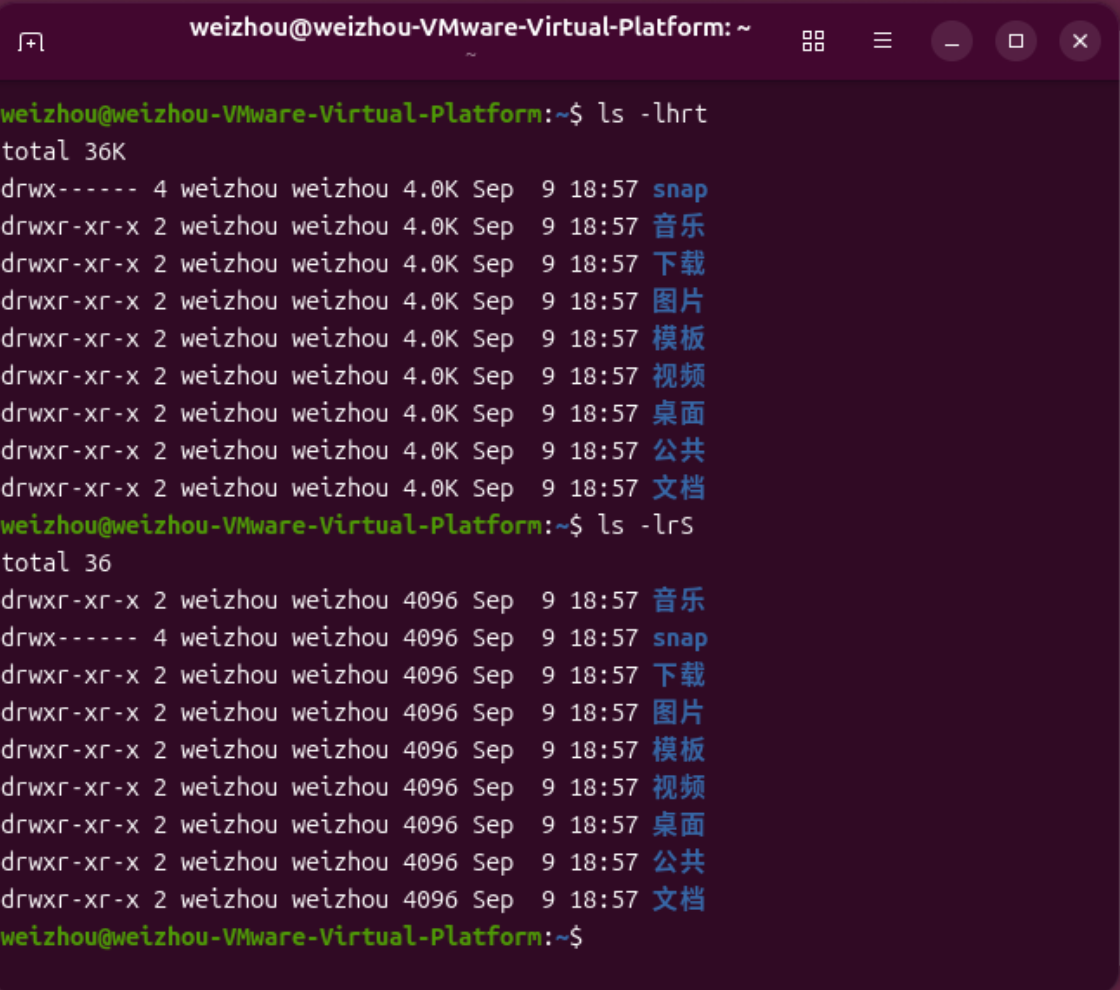
\includegraphics[width=0.8\textwidth]{Figure/ls命令示例}
  \caption{ls命令示例}
  \label{fig:ls命令示例}
\end{figure}

\subsection{cd 命令}
cd(changeDirectory) 命令语法：
\begin{lstlisting}[language=bash,title={cd(changeDirectory) 命令语法：}]
    cd [目录名]
\end{lstlisting}
说明：切换当前目录至 dirName。

示例：
\begin{lstlisting}[language=bash,title={进入要目录}]
    cd /
\end{lstlisting}
\begin{lstlisting}[language=bash,title={进入 "home" 目录}]
    cd ~
\end{lstlisting}
\begin{lstlisting}[language=bash,title={进入上一次工作路径}]
    cd -
\end{lstlisting}
\begin{lstlisting}[language=bash,title={把上个命令的参数作为cd参数使用。}]
    cd !$
\end{lstlisting}

\begin{figure}[h]
  \centering
  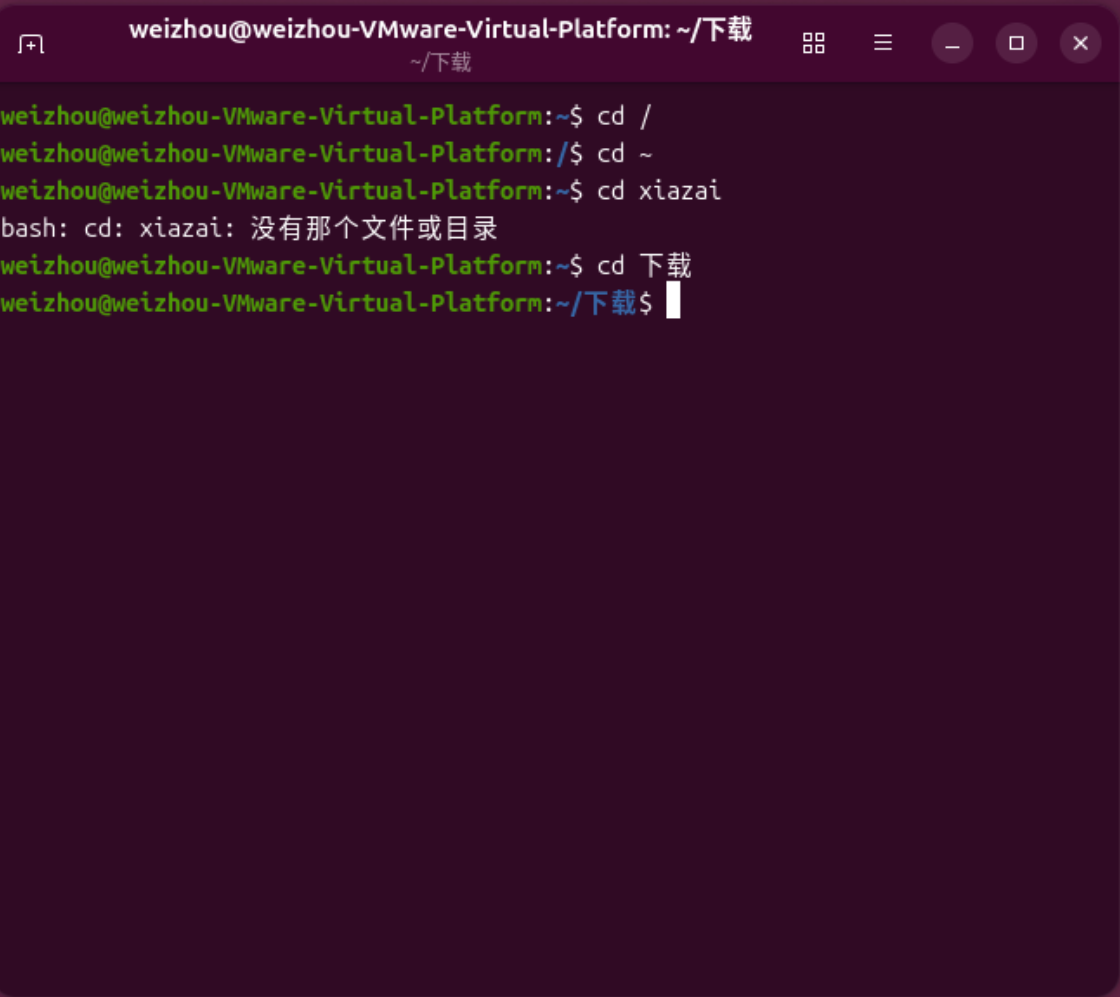
\includegraphics[width=0.8\textwidth]{Figure/cd命令示例}
  \caption{cd命令示例}
  \label{fig:cd命令示例}
\end{figure}

\subsection{pwd 命令}
pwd 命令用于查看当前工作目录路径。它是初学者最常用来确认``我现在在哪''的命令。
\begin{lstlisting}[language=bash,title={查看当前路径}]
    pwd
\end{lstlisting}
\begin{lstlisting}[language=bash,title={查看软链接的实际路径}]
    pwd -P
\end{lstlisting}
\begin{figure}[h]
  \centering
  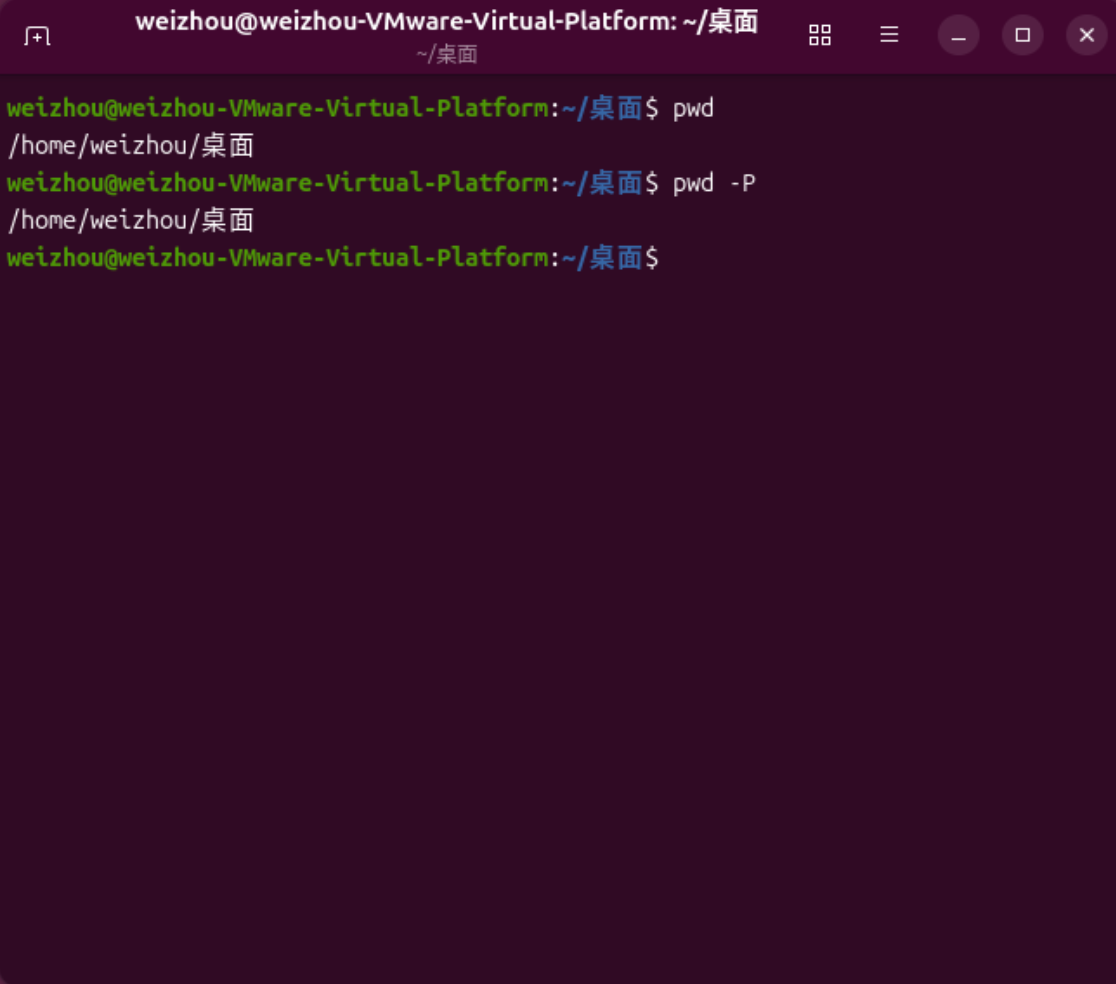
\includegraphics[width=0.8\textwidth]{Figure/pwd命令示例}
  \caption{pwd命令示例}
  \label{fig:pwd命令示例}
\end{figure}

\subsection{mkdir 命令}
mkdir 命令用于创建文件夹。
\begin{lstlisting}[language=bash,title={mkdir 常用参数}]
mkdir -m    对新建目录设置存取权限
mkdir -p    若路径中某些目录尚不存在, 系统会自动建立(一次建多级)
\end{lstlisting}
实例：
\begin{lstlisting}[language=bash,title={当前工作目录下创建名为 t 的文件夹}]
    mkdir t
\end{lstlisting}
\begin{lstlisting}[language=bash,title={在 tmp 下创建 path test/t1/t, 若目录不存在则一并建立}]
    mkdir -p /tmp/test/t1/t
\end{lstlisting}

\subsection{rm 命令}
删除一个或多个文件或目录。如果不加 \textit{-r} 选项，rm 不会删除目录。删除文件通常仍可以恢复，但删除目录需谨慎。
\begin{lstlisting}[language=bash,title={rm 常用参数}]
rm -i    删除前逐一询问确认
rm -r    递归删除(连同子目录一起删除)
rm -f    强制删除, 不提示
\end{lstlisting}
实例：
\begin{lstlisting}[language=bash,title={删除任何 .log 文件, 删除前逐一询问}]
    rm -i *.log
\end{lstlisting}
\begin{lstlisting}[language=bash,title={删除 test 子目录及其中所有内容, 不一一确认}]
    rm -rf test
\end{lstlisting}
\begin{lstlisting}[language=bash,title={删除以 - 开头的文件(用 -- 结束选项) }]
    rm -- -f*
\end{lstlisting}

\subsection{cp 命令}
将源文件复制到目标文件，或将多个源文件复制到目标目录。
\begin{lstlisting}[language=bash,title={cp 常用参数}]
cp -i    目标文件已存在时提示是否覆盖
cp -r    复制目录及目录内所有内容
cp -a    保持原文件的时间等属性
cp -s    建立符号链接(快捷方式)
\end{lstlisting}
实例：
\begin{lstlisting}[language=bash,title={复制 a.txt 到 test 目录, 保持时间, 存在则提示}]
    cp -ai a.txt test
\end{lstlisting}
\begin{lstlisting}[language=bash,title={为 a.txt 建立一个链接(快捷方式)}]
    cp -s a.txt link_a.txt
\end{lstlisting}

\subsection{mv 命令}
移动文件，或修改文件／目录名。当第二个参数是目录时，将第一个参数（可以是多个）移动到该目录。
\begin{lstlisting}[language=bash,title={mv 常用参数}]
mv -i    目标已存在时提示是否覆盖
\end{lstlisting}
实例：
\begin{lstlisting}[language=bash,title={将文件 test.log 改名为 test1.txt}]
    mv test.log test1.txt
\end{lstlisting}
\begin{lstlisting}[language=bash,title={把多个文件移动到根的 test3 目录}]
    mv log1.txt log2.txt log3.txt /test3
\end{lstlisting}
\begin{lstlisting}[language=bash,title={移动当前目录下所有文件到上一级目录}]
    mv * ../
\end{lstlisting}

\subsection{cat 命令}
cat 主要有三大功能：一次显示整个文件；从键盘创建一个新文件；将几个文件合并成一个文件。
\begin{lstlisting}[language=bash,title={cat 常用参数}]
cat -b    对非空输出行号
cat -n    输出所有行号
\end{lstlisting}
实例：
\begin{lstlisting}[language=bash,title={一次显示整个文件}]
    cat filename
\end{lstlisting}
\begin{lstlisting}[language=bash,title={从键盘创建一个文件(只能新建, 不能编辑已有文件)}]
    cat > filename
\end{lstlisting}
\begin{lstlisting}[language=bash,title={把 log2012.log 内容加上行号后写进 log2013.log}]
    cat -n log2012.log log2013.log
\end{lstlisting}
\begin{lstlisting}[language=bash,title={反向列示文件(与 cat 相反)}]
    tac log.txt
\end{lstlisting}

\subsection{more 命令}
功能类似于 cat，但会一页一页显示，方便逐页阅读。按空格键往下翻一页，按 \textit{b} 键往回翻一页，按 \textit{q} 键退出。
\begin{lstlisting}[language=bash,title={more 常用参数}]
more +n    从第 n 行开始显示
more -n    定义屏幕大小为 n 行
more -s    把连续多个空行显示为一行
\end{lstlisting}
实例：
\begin{lstlisting}[language=bash,title={显示文件中从第 3 行起的内容}]
    more +3 text.txt
\end{lstlisting}
\begin{lstlisting}[language=bash,title={借助管道让 ls -l 每次只显示 5 行}]
    ls -l | more -5
\end{lstlisting}

\subsection{less 命令}
less 与 more 类似，但使用 less 可以随意前后浏览文件，more 只能向前。而且 less 在查看之前不会加载整个文件，更适合大文件。
\begin{lstlisting}[language=bash,title={less 常用操作}]
/字符串    向下搜索字符串
?字符串    向上搜索字符串
n          重复前一个搜索
N          反向重复前一个搜索
空格        滚动一页
b          向后翻一页
-q         退出
\end{lstlisting}
实例：
\begin{lstlisting}[language=bash,title={查看进程信息并通过 less 分页显示(带行号)}]
    ps -aux | less -N
\end{lstlisting}
\begin{lstlisting}[language=bash,title={查看多个文件(按 n 下一个, p 前一个)}]
    less 1.log 2.log
\end{lstlisting}

\subsection{head 命令}
显示文件的开头内容，默认显示前 10 行。
\begin{lstlisting}[language=bash,title={head 常用参数}]
head -n <行数>    显示的行数
head -c <字节数>  显示前多少个字节
\end{lstlisting}
实例：
\begin{lstlisting}[language=bash,title={显示 1.log 文件中前 20 行}]
    head 1.log -n 20
\end{lstlisting}
\begin{lstlisting}[language=bash,title={显示最后 10 行(行数为负数表示从后往前数)}]
    head -n -10 t.log
\end{lstlisting}

\subsection{tail 命令}
显示文件末尾内容，常用来查看日志文件。
\begin{lstlisting}[language=bash,title={tail 常用参数}]
tail -f    循环读取(适合查看动态增加的日志)
tail -n <行数>  显示行数(从后往前)
\end{lstlisting}
实例：
\begin{lstlisting}[language=bash,title={循环读取逐渐增加的文件内容}]
    tail -f ping.log
\end{lstlisting}

\subsection{which、whereis、locate、find 命令}
这四个命令都能用来找文件，但原理和适用场景各不相同：
\begin{itemize}
    \item \textbf{which} 在 PATH 中查找可执行命令的位置，返回第一个匹配结果。
    \item \textbf{whereis} 只搜索程序名相关的二进制、帮助和源码文件，速度快。
    \item \textbf{locate} 基于系统数据库查找文件，速度很快，但新建文件可能找不到。
    \item \textbf{find} 实际遍历硬盘查找文件，最准确但最慢。
\end{itemize}
实例：
\begin{lstlisting}[language=bash,title={查看 ls 命令是否存在及其位置}]
    which ls
\end{lstlisting}
\begin{lstlisting}[language=bash,title={查找 locate 程序的相关文件}]
    whereis locate
\end{lstlisting}
\begin{lstlisting}[language=bash,title={查找与 pwd 相关的所有文件}]
    locate pwd
\end{lstlisting}
\begin{lstlisting}[language=bash,title={在当前目录查找以 .log 结尾的文件}]
    find ./ -name '*.log'
\end{lstlisting}
\begin{lstlisting}[language=bash,title={查找 /opt 目录下权限为 777 的文件}]
    find /opt -perm 777
\end{lstlisting}
\begin{lstlisting}[language=bash,title={查找更改时间在 10 日以前的文件并删除(无提示)}]
    find . -type f -mtime +10 -exec rm -f {} \;
\end{lstlisting}

\subsection{grep 命令}
强大的文本搜索命令，全称 Global Regular Expression Print，即全局正则表达式搜索。它在文件或多个文件中搜索字符串模板，结果输出到标准输出，不改变原文件内容。
\begin{lstlisting}[language=bash,title={grep 常用参数}]
grep -c    计算符合样式的列数
grep -i    忽略大小写
grep -l    只列出文件名
grep -n    显示匹配行所在行号
grep -R    递归查找文件夹
\end{lstlisting}
实例：
\begin{lstlisting}[language=bash,title={查找指定进程}]
    ps -ef | grep svn
\end{lstlisting}
\begin{lstlisting}[language=bash,title={从文件夹递归查找以 grep 开头的行, 只列出文件}]
    grep -lR '^grep' /tmp
\end{lstlisting}
\begin{lstlisting}[language=bash,title={显示包含 ed 或 at 内容的行为}]
    grep -E 'ed|at' test.txt
\end{lstlisting}

\subsection{wc 命令}
wc(word count) 用于统计指定文件中字节数、单词数、行数，并将统计结果输出。
\begin{lstlisting}[language=bash,title={wc 常用参数}]
wc -c    统计字节数
wc -l    统计行数
wc -m    统计字符数
wc -w    统计单词数
\end{lstlisting}
实例：
\begin{lstlisting}[language=bash,title={统计文件的 行数 单词数 字节数}]
    wc text.txt
\end{lstlisting}
\begin{lstlisting}[language=bash,title={统计输出的行数}]
    cat test.txt | wc -l
\end{lstlisting}

\subsection{chmod 命令}
用于改变 Linux 系统文件或目录的访问权限。权限用 r(读)、w(写)、x(执行)表示，对应数字为 4、2、1。每一文件有三组权限：属主、属组、其他用户。
\begin{lstlisting}[language=bash,title={chmod 常用参数}]
chmod -R    递归处理目录及子目录下所有文件
\end{lstlisting}
权限代号：
\begin{lstlisting}[language=bash,title={权限数字对应}]
r = 4    读
w = 2    写
x = 1    执行
\end{lstlisting}
实例：
\begin{lstlisting}[language=bash,title={增加文件 t.log 所有用户的可执行权限}]
    chmod a+x t.log
\end{lstlisting}
\begin{lstlisting}[language=bash,title={属主读写执行(7), 属组读执行(5), 其他执行(1)}]
    chmod 751 t.log
\end{lstlisting}
\begin{lstlisting}[language=bash,title={将 test 目录及子目录所有文件添加可读权限}]
    chmod u+r,g+r,o+r -R text/
\end{lstlisting}

\subsection{tar 命令}
用来打包和解压文件。注意 tar 本身只打包不压缩，压缩与解压是调用其他工具（如 gzip、bzip2）完成的。常用的两招是 \textit{tar zcvf} 打包压缩、\textit{tar zxvf} 解压。
\begin{lstlisting}[language=bash,title={tar 常用参数}]
-c    建立新的压缩文件
-x    从压缩包中解压
-t    显示压缩文件中的内容
-z    支持 gzip 压缩
-j    支持 bzip2 压缩
-v    显示操作过程
-f    指定压缩文件名
\end{lstlisting}
实例：
\begin{lstlisting}[language=bash,title={将文件全部打包成 tar 包}]
    tar -cvf log.tar log1.log log2.log
\end{lstlisting}
\begin{lstlisting}[language=bash,title={将 /etc 下所有文件和目录打包并用 gz 压缩}]
    tar -zcvf /tmp/etc.tar.gz /etc
\end{lstlisting}
\begin{lstlisting}[language=bash,title={查看刚打包的文件内容(必须加 z, 因为用 gzip 压缩)}]
    tar -ztvf /tmp/etc.tar.gz
\end{lstlisting}
\begin{lstlisting}[language=bash,title={解压}]
    tar -zxvf filename.tar.gz
\end{lstlisting}

\subsection{ps 命令}
ps(process status) 用来查看当前运行的进程状态，一次性查看。如需动态连续结果，用 \textit{top}。
\begin{lstlisting}[language=bash,title={ps 常用参数}]
ps -A    显示所有进程
ps -e    显示所有进程(等同 -A)
ps -f    显示进程间的关系(完整格式)
ps -aux  显示所有包含其他信息的进程
\end{lstlisting}
实例：
\begin{lstlisting}[language=bash,title={显示当前所有进程环境变量及进程间关系}]
    ps -ef
\end{lstlisting}
\begin{lstlisting}[language=bash,title={与 grep 联用查找某进程}]
    ps -aux | grep apache
\end{lstlisting}

\subsection{top 命令}
动态显示当前系统正在执行的进程信息，包括进程 ID、CPU 占用率、内存占用率等。交互界面里按 \textit{q} 退出。
\begin{lstlisting}[language=bash,title={top 常用参数}]
top -p <进程号>    指定进程显示
top -n <次数>      循环显示次数
\end{lstlisting}
\begin{lstlisting}[language=bash,title={top 交互命令}]
P    按 CPU 使用率排序
M    按内存使用率排序
q    退出
\end{lstlisting}

\subsection{free 命令}
显示系统内存使用情况，包括物理内存、交换区内存(swap)和内核缓冲区内存。
\begin{lstlisting}[language=bash,title={free 常用参数}]
free -m    以 MB 为单位显示
free -g    以 GB 为单位显示
free -s <秒>  每隔多少秒持续显示
\end{lstlisting}
实例：
\begin{lstlisting}[language=bash,title={显示内存使用情况}]
    free -m
\end{lstlisting}

\subsection{df 命令}
显示磁盘空间使用情况，获取硬盘已占用多少、还剩多少等信息。
\begin{lstlisting}[language=bash,title={df 常用参数}]
df -h    以易读方式显示
df -T    列出文件系统类型
df -a    全部文件系统列表
\end{lstlisting}
实例：
\begin{lstlisting}[language=bash,title={以易读方式列出所有文件系统及其类型}]
    df -haT
\end{lstlisting}

\subsection{du 命令}
查看文件和目录的磁盘使用空间，与 df 不同，du 针对的是具体文件或目录。
\begin{lstlisting}[language=bash,title={du 常用参数}]
du -h    以易读方式显示文件大小
du -s    仅显示总计
du -a    显示目录中所有文件大小
\end{lstlisting}
实例：
\begin{lstlisting}[language=bash,title={以易读方式显示文件夹内及子文件夹大小}]
    du -h scf/
\end{lstlisting}
\begin{lstlisting}[language=bash,title={显示几个文件各自占用空间并统计总和}]
    du -hc test/ scf/
\end{lstlisting}

\subsection{ln 命令}
为文件在另一个位置建立一个链接。软链接(\textit{ln -s})类似于 Windows 里的快捷方式，可跨文件系统、可用于目录；硬链接(\textit{ln})以文件副本形式存在，但同一文件系统内才可创建，且不占用实际空间。无论改哪一处，其余链接都会同步变化。
\begin{lstlisting}[language=bash,title={ln 常用参数}]
ln -s    软链接(符号链接)
ln -v    显示详细处理过程
\end{lstlisting}
实例：
\begin{lstlisting}[language=bash,title={给文件创建软链接并显示操作信息}]
    ln -sv source.log link.log
\end{lstlisting}

\subsection{date 与 cal 命令}
date 显示或设定系统的日期与时间；cal 显示公历（阳历）日历。
\begin{lstlisting}[language=bash,title={date 常用格式}]
%Y    年份(四位数)
%m    月份(01-12)
%d    日期(01-31)
%H    小时(00-23)
%M    分钟(00-59)
\end{lstlisting}
实例：
\begin{lstlisting}[language=bash,title={显示指定日期格式}]
    date +%Y%m%d
\end{lstlisting}
\begin{lstlisting}[language=bash,title={显示下一天}]
    date -d "+1 day" +%Y%m%d
\end{lstlisting}
\begin{lstlisting}[language=bash,title={显示 2013 年每个月的日历}]
    cal -y 2013
\end{lstlisting}
\begin{lstlisting}[language=bash,title={将星期一作为第一列, 显示前中后三月}]
    cal -3m
\end{lstlisting}

\subsection{kill 命令}
发送指定信号给相应进程。默认发送 SIGTERM(15) 终止指定进程，若无法终止可用 \textit{-KILL}（发送 SIGKILL，9）强制结束进程。用 ps 或 jobs 查看进程号；root 用户可影响所有用户的进程，普通用户只能影响自己。
\begin{lstlisting}[language=bash,title={kill 常用参数}]
kill -l           列出全部信号名称
kill -9 <PID>     强制结束进程
\end{lstlisting}
实例：
\begin{lstlisting}[language=bash,title={先查找进程 pro1, 然后强制杀掉}]
    kill -9 $(ps -ef | grep pro1)
\end{lstlisting}

\section{鱼香ROS的指令}
上面的是Linux的常用指令，下面一个指令非常重要，是咱们使用ROS系统可以会的指令，极大节省时间：
\begin{lstlisting}[language=bash,title={一键安装}]
    wget http://fishros.com/install -O fishros && . fishros
\end{lstlisting}
这条指令来自我关注的博主“鱼香ROS”，非常好用。效果如下图：
\begin{figure}[h]
  \centering
  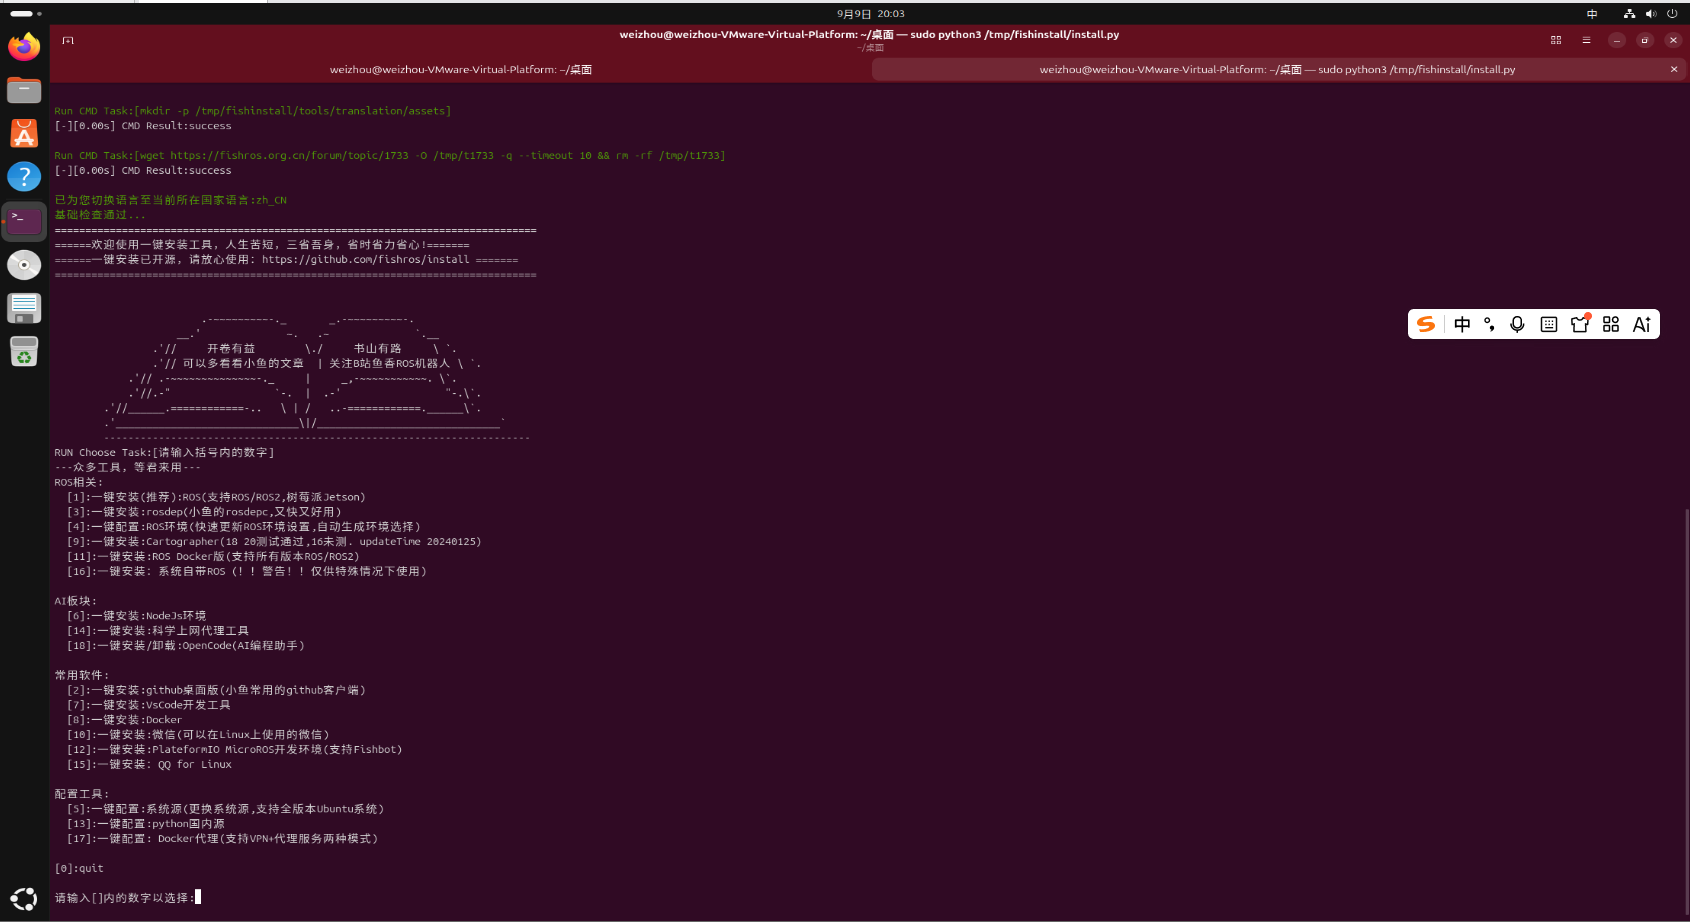
\includegraphics[width=0.6\textwidth]{Figure/小鱼的一键安装命令.png}
  \caption{小鱼的一键安装命令}
  \label{fig:小鱼的一键安装命令}
\end{figure}
显然，包含了咱们要用的几乎所有工具。

\section{用自然语言来使用Unbuntu}
AI时代，古法编程的艺术仍在流传，但Vibe Coding已经成为主流。我选择在保留自己读写代码能力的同时，先装一个npm,再装上opencode，然后美美使用中文使用Unbuntu（doge）
\begin{figure}[h]
  \centering
  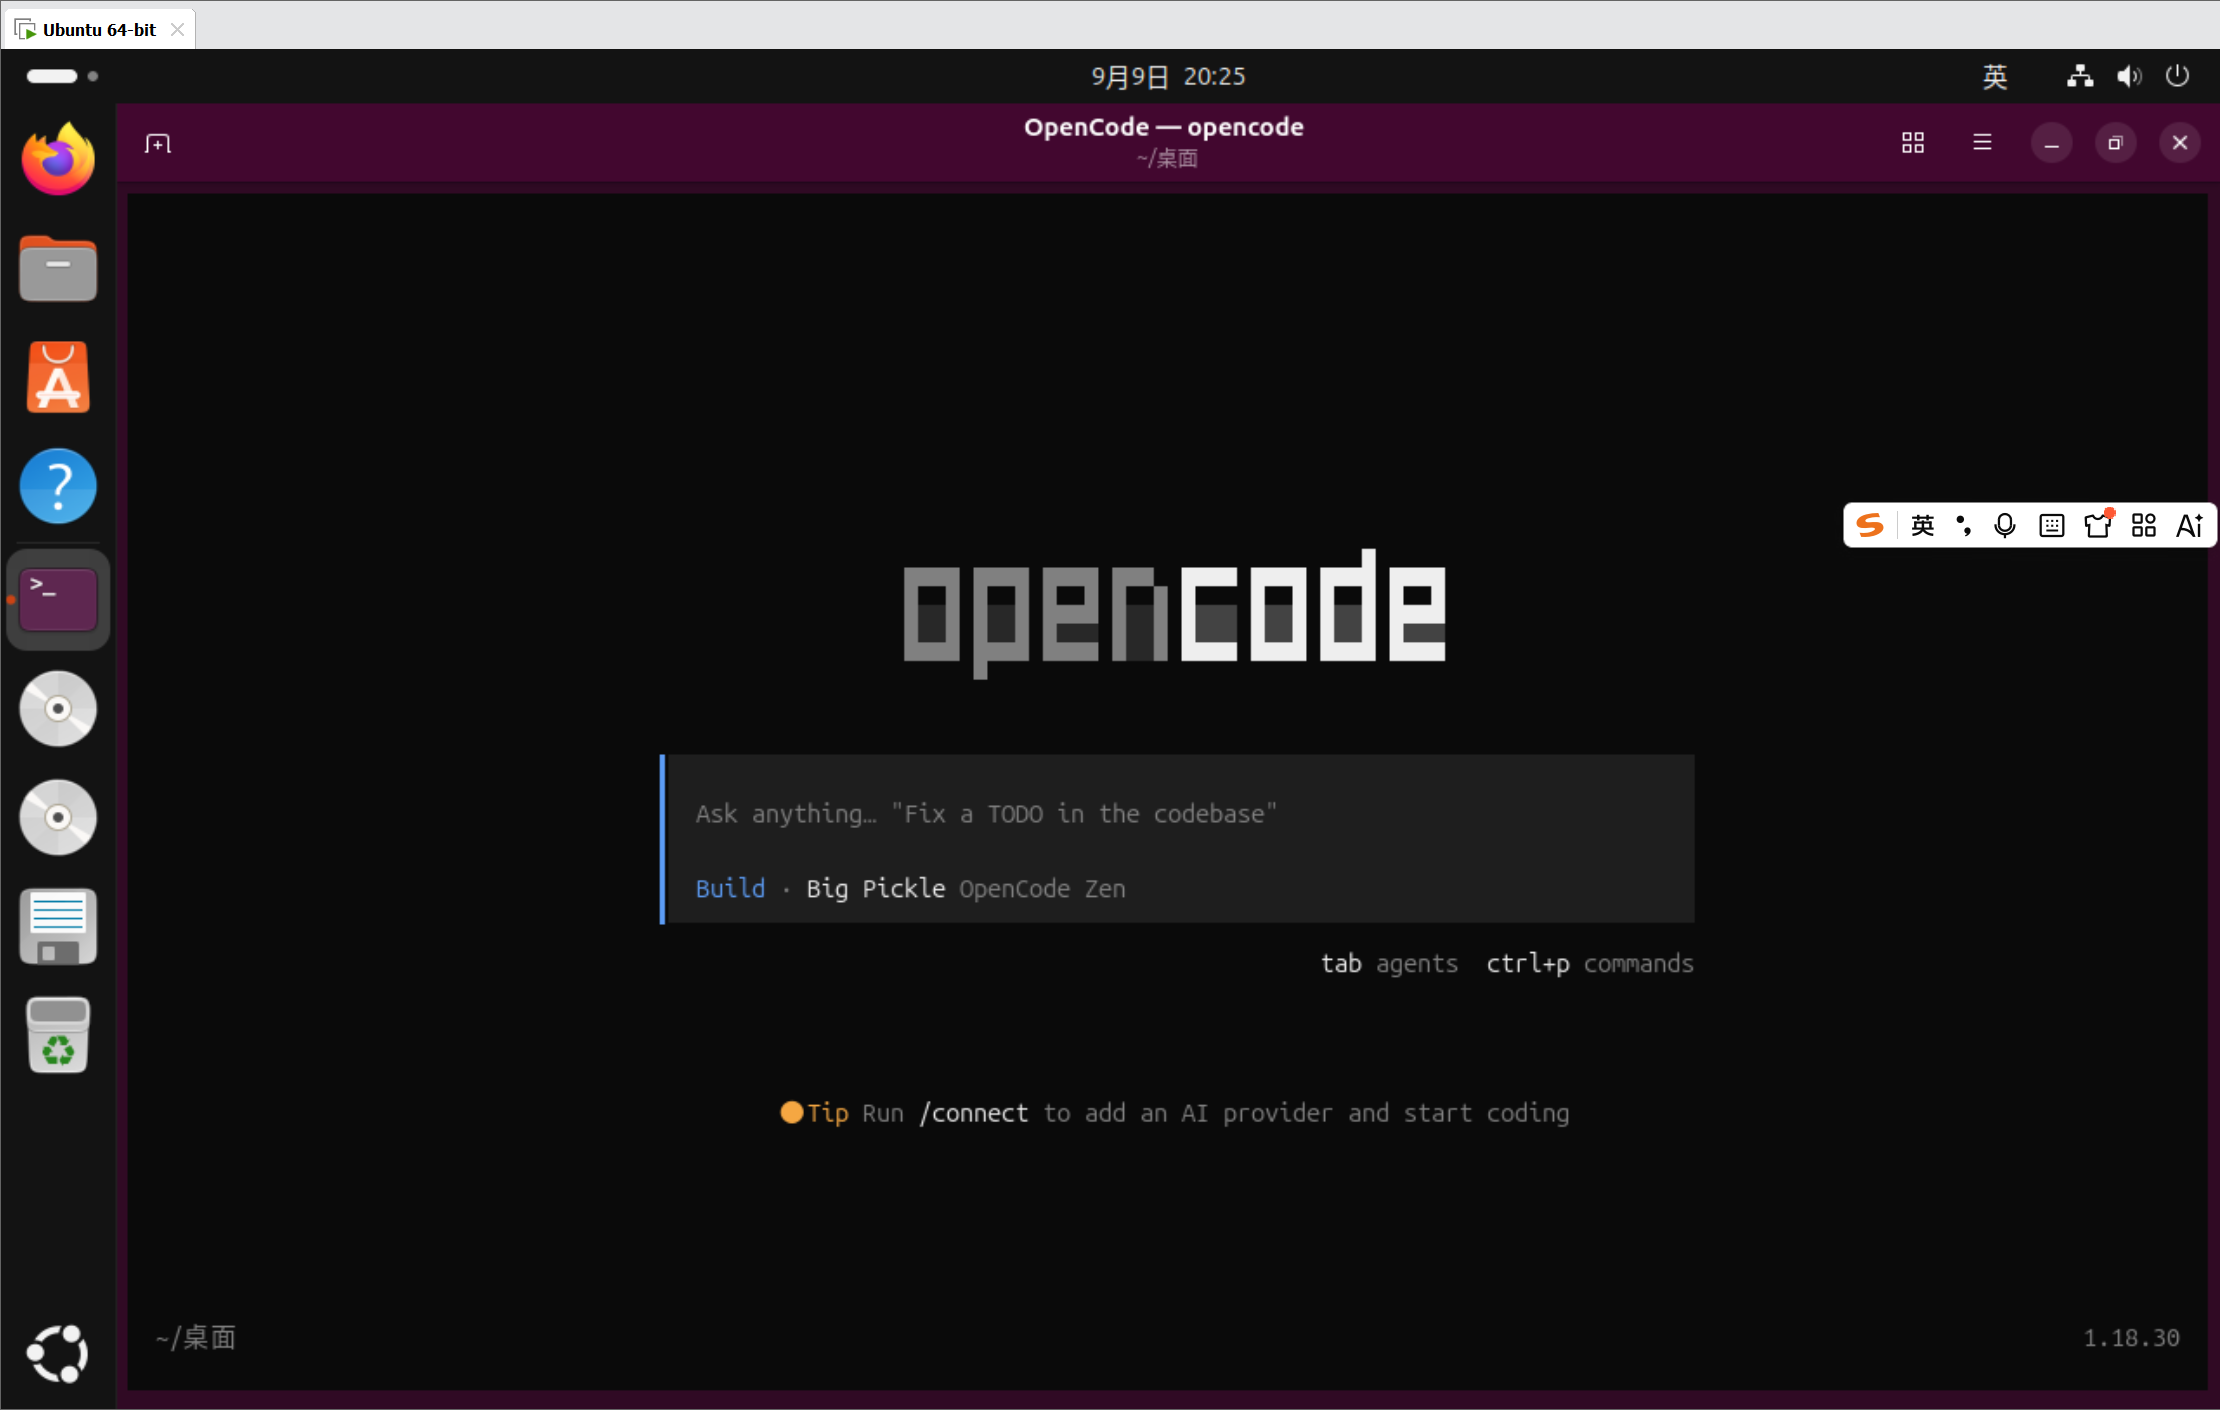
\includegraphics[width=0.8\textwidth]{Figure/Unbuntu中的opencode.png}
  \caption{Unbuntu中的opencode}
  \label{fig:Unbuntu中的opencode}
\end{figure}

% ============ 文件结尾 ============
% 整书模式(被 main.tex 引用): 读到这里即 \endinput 交还控制权,
% 不会执行下方的 \end{document}。
\ifcsname wholebook\endcsname
\expandafter\endinput
\fi

% 单独编译模式: 在顶层(无未闭合条件)执行 \end{document} 收尾。
\end{document}
